\subsection{Sentiment Analysis}
\label{sec:sentiment_analysis}

The sentiment analysis examines 29,096 sentences extracted from all the stores. For each sentence, a compound score was calculated. Additionally, the proportion of negativity, neutrality and positivity of each sentence was also calculated.

Neutral sentiment sentences have a compound score of 0. Negative compound scores are considered to be a negative sentiment, and values higher than 0 are considered to be positive. Table \ref{tab:sentiment_proportion} shows the proportion of each sentiment in the data sets.

\begin{table}
    \centering
    \begin{tabular}{llll}
        \hline
        Data set & Positive & Neutral & Negative \\ \hline
        With spell-correction & 0.31 & 0.41 & 0.23 \\
        Without spell-correction & 0.31 & 0.42 & 0.27 \\
        \hline
    \end{tabular}
    \caption{Proportion of sentiments in the data sets. Values are rounded to two decimal places.}
    \label{tab:sentiment_proportion}
\end{table}

The mean compound score of the data set with spell-correct is 0.00 with a standard deviation of 0.35, while that of the set without spell-correct is also 0.00 with a standard deviation of 0.35. Figure \ref{fig:sentiment_distribution} shows the distribution of the compound scores in both data sets and table \ref{tab:sentiment_analysis} shows a summary of the distribution that includes the maximum and minimum values.

\begin{figure}[H]
    \centering
    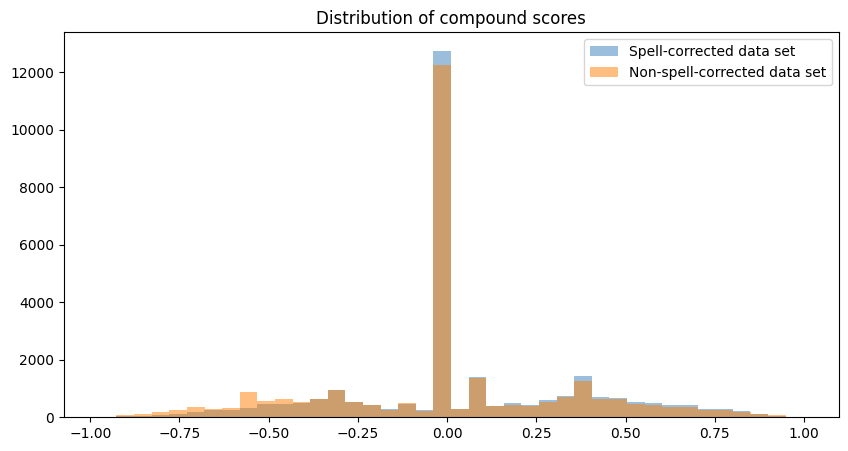
\includegraphics[width=\textwidth]{resources/compound_scores.png}
    \caption{Distribution of the compound scores in the data sets.}
    \label{fig:sentiment_distribution}
\end{figure}

\begin{table}
    \centering
    \resizebox*{\textwidth}{!}{
        \begin{tabular}{lcccc}
            \hline
            Data set & Mean & Standard deviation & Minimum & Maximum \\ \hline
            With spell-correction & 0.00 & 0.35 & -0.98 & 1.00 \\
            Without spell-correction & 0.00 & 0.35 & -0.98 & 1.00 \\
            \hline
        \end{tabular}
    }
    \caption{Description of the sentiment analyses distributions.}
    \label{tab:sentiment_analysis}
\end{table}

The distribution of the negativity proportions in sentences is shown in figure \ref{fig:negativity_distribution}.

\begin{figure}[H]
    \centering
    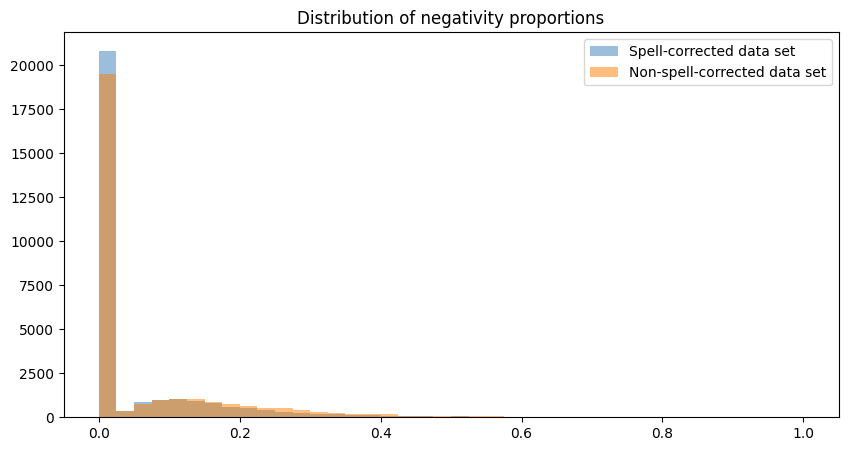
\includegraphics[width=\textwidth]{resources/negativity_distributions.png}
    \caption{Distribution of the negativity proportions in the data sets.}
    \label{fig:negativity_distribution}
\end{figure}

The non-spell-corrected data set contains 9,619 with negativity proportions larger than 0, while the spell-corrected data set contains 9,706. This is a difference of 87 sentences.

The positivity proportions are presented in the same fashion in figure \ref{fig:positivity_distribution}.

The non-spell-corrected data set contains 11,443 sentences with positivity proportions larger than 0, while the spell-corrected data set contains 11,579. The spell-corrected data set contains 136 more sentences with positive proportions.

The non-spell-corrected data set has 1,160 more positive sentences than negative sentences, meaning sentences with compound scores over 0, while the spell-corrected data set has 1,170 more positive sentences than negative sentences.


\begin{figure}[H]
    \centering
    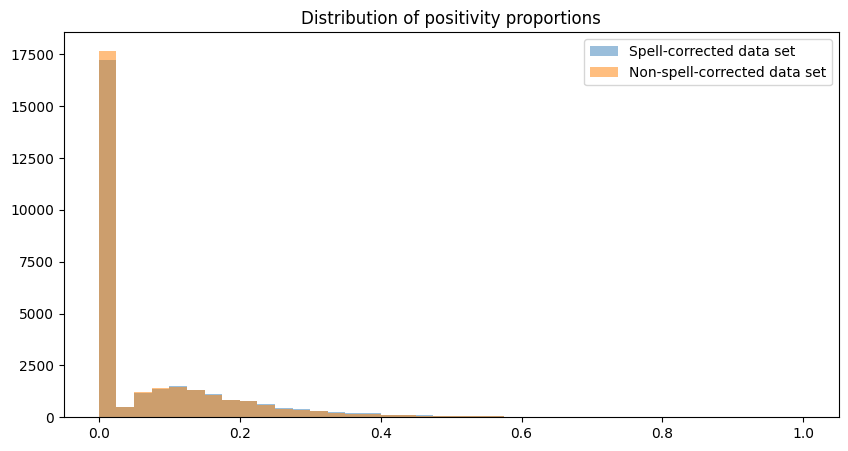
\includegraphics[width=1\textwidth]{resources/positivity_distributions.png}
    \caption{Distribution of the positivity proportions in the data sets.}
    \label{fig:positivity_distribution}
\end{figure}

The distributions of all proportions are visually shown in figure \ref{fig:proportions}.

\begin{figure}[H]
    \centering
    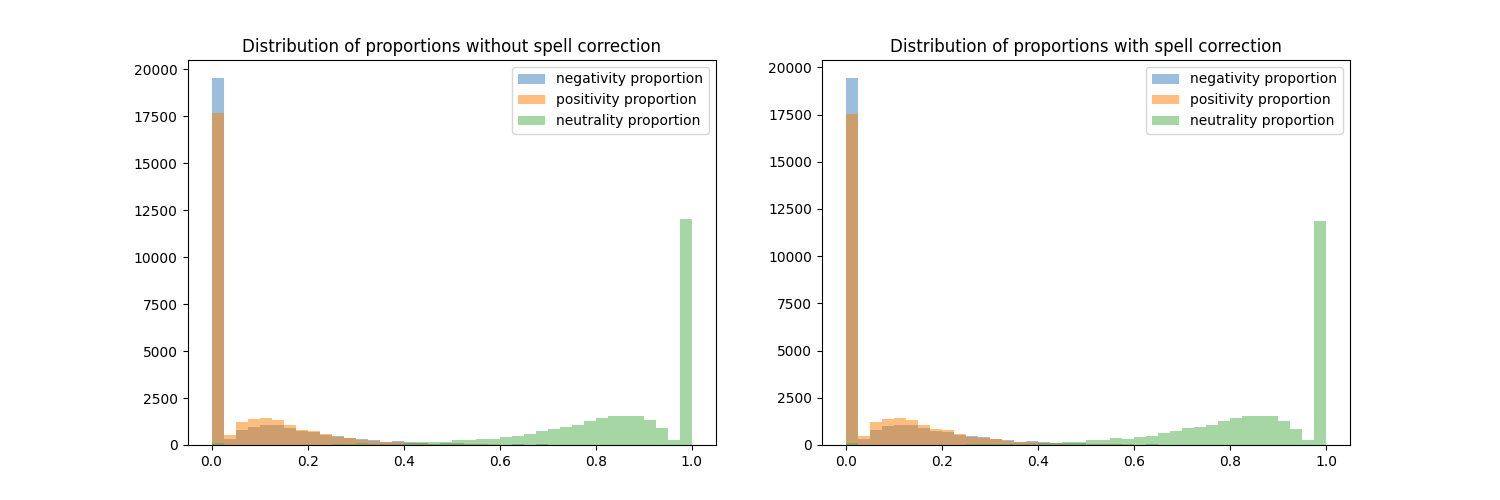
\includegraphics[width=1\textwidth]{resources/proportions.png}
    \caption{Distribution of the positivity proportions in the data sets.}
    \label{fig:proportions}
\end{figure}